\documentclass[12pt]{article}

% Page geometry
\usepackage[margin=1in]{geometry}

% Packages
\usepackage{graphicx}
\usepackage{amsmath, amssymb}
\usepackage{booktabs}
\usepackage{hyperref}
\usepackage{float}
\usepackage{caption}
\usepackage{subcaption}
\usepackage{natbib}
\usepackage{xcolor}
\usepackage{enumitem}

% Brand colors
\definecolor{garnet}{HTML}{73000A}
\definecolor{atlantic}{HTML}{466A9F}
\definecolor{congaree}{HTML}{1F414D}

% Hyperlink styling
\hypersetup{
    colorlinks=true,
    linkcolor=garnet,
    citecolor=atlantic,
    urlcolor=congaree
}

% Bibliography style
\bibliographystyle{plainnat}

\begin{document}

% ============================================================
% HEADER
% ============================================================
\begin{center}
    {\large \textbf{CSCE 775: Deep Reinforcement Learning and Search}} \\[0.5em]
    {\LARGE \textbf{RL-Optimized Multimodal Registration and\\Augmentation Policy for IR/RGB Perception}} \\[1em]
    {\large Jacob Whisenant, Xeerak Muhammed, J.C. Vaught} \\[0.5em]
    {\large February 13, 2026}
\end{center}

\vspace{1em}

% ============================================================
% INTRODUCTION
% ============================================================
\section{Introduction}

Autonomous systems operating in unstructured environments---such as unmanned surface vehicles navigating lakes, rivers, and coastal waters---rely on multimodal perception to maintain situational awareness across diverse and degraded conditions. Infrared (IR) and visible (RGB) cameras provide complementary information. RGB sensors capture rich texture and color detail under adequate illumination, while IR sensors detect thermal signatures that persist through fog, rain, darkness, and glare \citep{Ma2022ImageFusion}. Fusing these modalities requires accurate spatial registration (geometric alignment) and appropriate data augmentation during training to build robust downstream models for detection, tracking, and segmentation \citep{Zhang2023DeepFusion, Zhao2023CDDFuse}. However, the optimal registration transform and augmentation strategy depend heavily on scene context, including sensor pose changes, environmental conditions, and domain-specific characteristics of different water-body types. Figure~\ref{fig:weather} illustrates this challenge: RGB image quality degrades significantly under adverse weather and lighting, while IR imagery remains relatively stable, creating a shifting alignment and fusion problem that static pipelines cannot adequately address.

\begin{figure}[H]
    \centering
    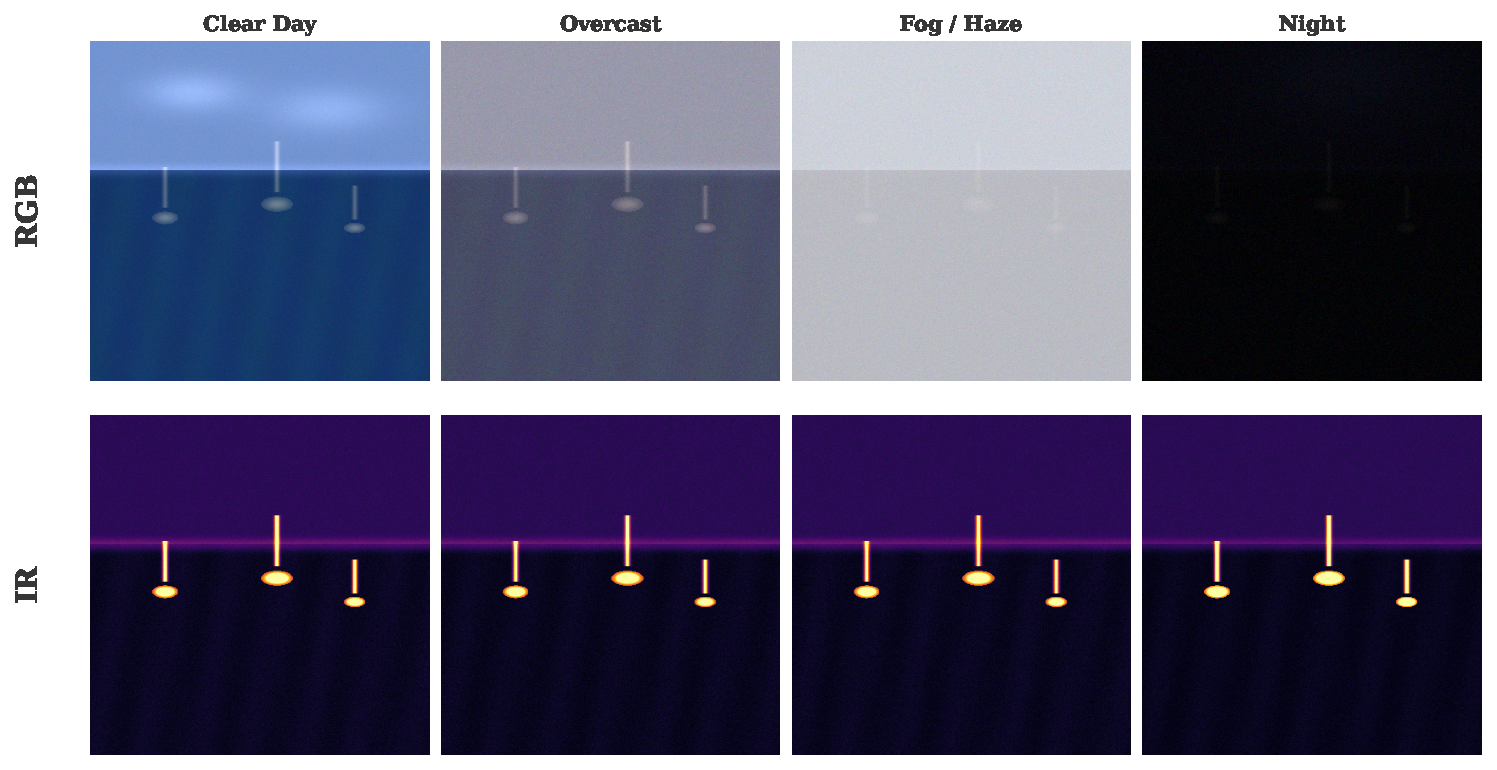
\includegraphics[width=\textwidth]{figures/fig7_weather_conditions.pdf}
    \caption{The multimodal perception challenge across environmental conditions. RGB imagery (top row) degrades substantially under overcast, fog, and night conditions, while IR imagery (bottom row) maintains consistent scene representation. This asymmetric degradation means the optimal registration and augmentation strategy must adapt to current conditions.}
    \label{fig:weather}
\end{figure}

Current approaches to multimodal registration and augmentation suffer from a fundamental rigidity. Classical registration pipelines apply a fixed transform family (e.g., affine or homography) regardless of scene content, while learned registration networks \citep{Balakrishnan2019VoxelMorph, DeVos2019RLRegistration} are trained with a single augmentation recipe that may not generalize across domains. Data augmentation strategies are typically hand-designed or selected via expensive grid searches. AutoAugment \citep{Cubuk2019AutoAugment} demonstrated that reinforcement learning can discover augmentation policies that outperform human-designed strategies, but it operates on single-modality images and does not account for the registration step. We propose to unify registration transform selection and augmentation policy optimization into a single RL framework. The agent learns to jointly select the registration method, its parameters, and the augmentation recipe conditioned on frame quality cues, alignment residuals, and environment type, maximizing downstream perception performance as its reward signal.

% ============================================================
% APPROACH
% ============================================================
\section{Approach}

\subsection{Related Work}

\textbf{Image Registration.} Image registration aligns two or more images into a common coordinate frame. For multimodal IR/RGB registration, classical methods rely on feature matching (SIFT, SURF) followed by homography estimation, but these struggle when modalities share few common features \citep{Ma2022ImageFusion}. Deep learning approaches learn registration end-to-end. VoxelMorph \citep{Balakrishnan2019VoxelMorph} introduced a CNN-based framework for deformable registration in medical imaging, while de Vos et al. \citep{DeVos2019RLRegistration} proposed unsupervised affine and deformable registration networks. SuperFusion \citep{Tang2022SuperFusion} jointly performs registration and fusion with semantic awareness, showing that coupling these stages improves downstream performance. However, all of these methods use a fixed architecture and training regime, without adapting their strategy to scene conditions at inference time.

\textbf{RL for Registration.} Reinforcement learning has been applied to image registration in medical imaging. Liao et al. \citep{Liao2017ArtificialAgent} trained an artificial agent to perform rigid registration by iteratively predicting transform updates, treating registration as a sequential decision problem. Krebs et al. \citep{Krebs2017RobustRL} extended this to non-rigid registration with agent-based action learning, achieving robust alignment under anatomical variability. These works demonstrate that RL can handle the sequential, decision-dependent nature of registration, but they have not been applied to the multimodal IR/RGB setting or combined with augmentation policy optimization.

\textbf{RL for Augmentation Policies.} AutoAugment \citep{Cubuk2019AutoAugment} used a recurrent neural network controller trained with REINFORCE to search over augmentation policies, achieving state-of-the-art results on CIFAR-10 and ImageNet. Fast AutoAugment \citep{Lim2019FastAutoAugment} and Faster AutoAugment \citep{Hataya2020FasterAutoAugment} reduced the search cost through density matching and gradient-based optimization, respectively. RandAugment \citep{Cubuk2020RandAugment} simplified the search space to just two hyperparameters. While these methods are effective for single-modality classification, none addresses the unique challenges of multimodal augmentation, where augmentations must be \textit{coordinated} across modalities to preserve alignment consistency.

\textbf{RL for Vision Pipelines.} AdaptiveISP \citep{Wang2024AdaptiveISP} demonstrated that deep RL can optimize an entire image signal processing pipeline for object detection, dynamically selecting ISP operations and parameters based on scene content. Active Domain Randomization \citep{Mehta2020ActiveDR} uses RL to select simulator parameters that maximize environment informativeness for policy transfer. These works motivate our approach: if RL can optimize ISP pipelines and simulator configurations, it can also optimize the registration-plus-augmentation pipeline that sits between raw sensor data and downstream perception models.

\textbf{Domain Adaptation for Multimodal Perception.} Domain-adversarial training \citep{Ganin2016DomainAdversarial} learns domain-invariant features but does not modify the input pipeline. Transfer learning surveys for vehicle perception \citep{Liu2023TransferVehicle} highlight the persistent domain gap across weather conditions, sensor configurations, and geographic regions. RGB-T tracking benchmarks such as LasHeR \citep{Li2022RGBTTracking} and RGBT234 \citep{Li2023IRRegistration} demonstrate that multimodal approaches outperform single-modality methods, but performance varies significantly across conditions, motivating an adaptive approach.

\subsection{MDP Formulation}

We formulate the joint registration and augmentation optimization as a Markov Decision Process (MDP). At each training step $t$, the RL agent observes a state, selects an action, and receives a reward based on downstream perception performance. Figure~\ref{fig:architecture} presents the complete system architecture, and Figure~\ref{fig:mdp} details the MDP formulation.

\begin{figure}[H]
    \centering
    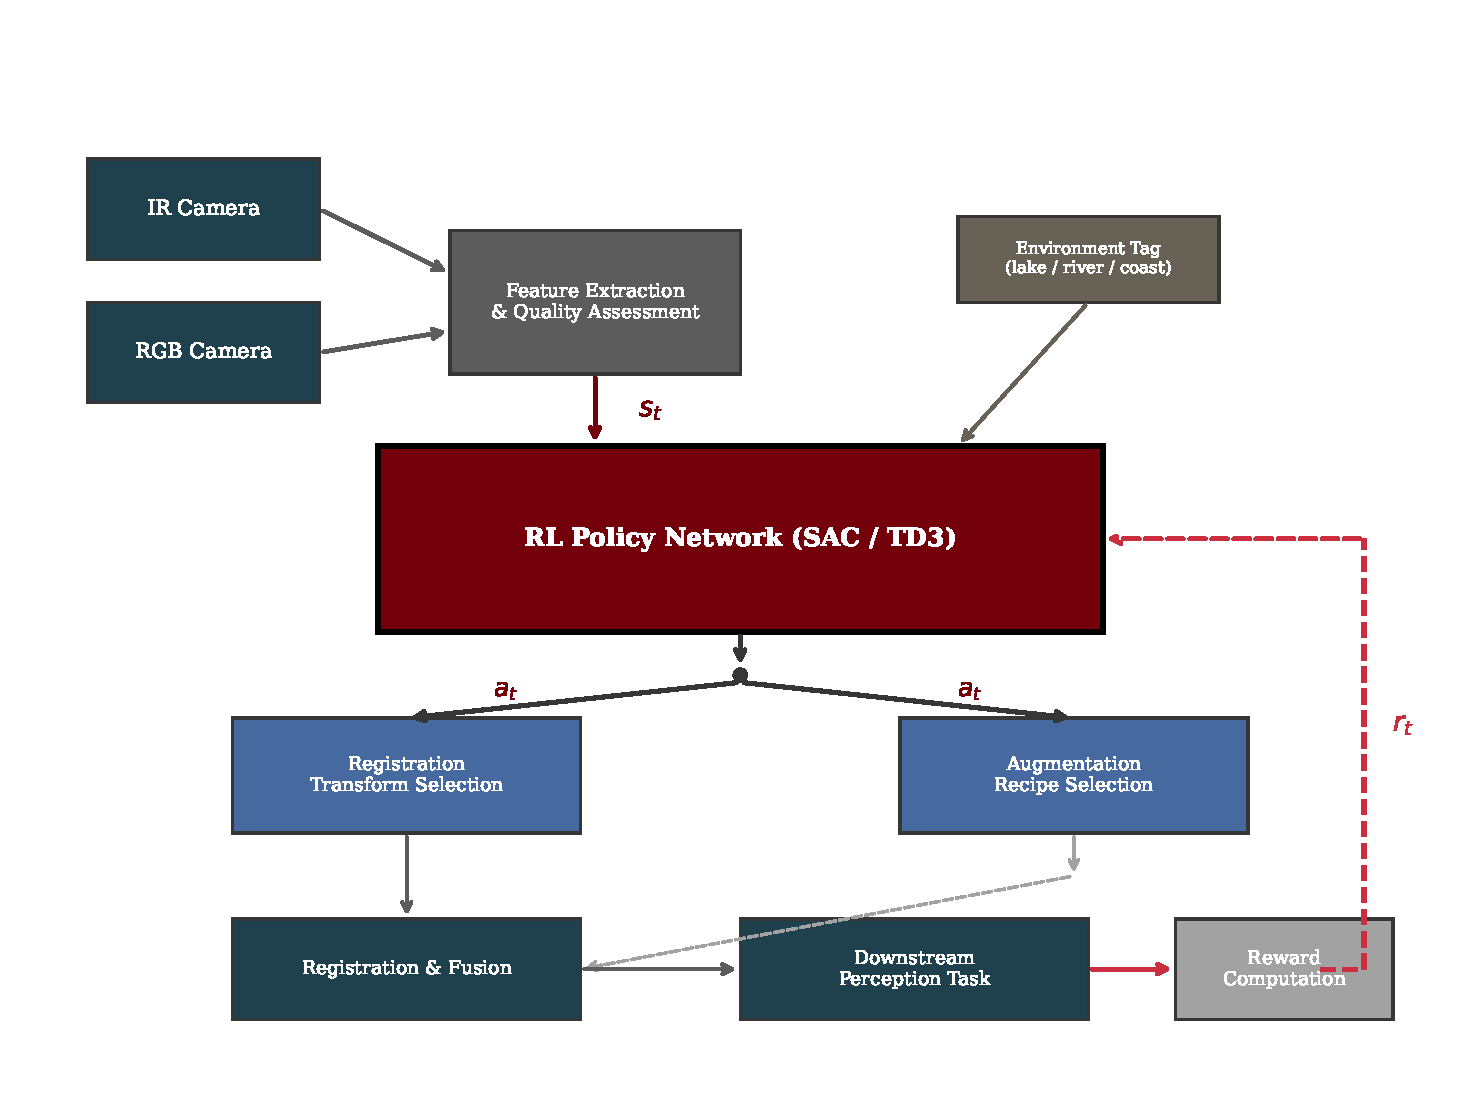
\includegraphics[width=\textwidth]{figures/fig1_system_architecture.pdf}
    \caption{System architecture. IR and RGB inputs are processed through feature extraction and quality assessment to form the state $s_t$. The RL policy network outputs actions $a_t$ comprising registration transform selection and augmentation recipe. The registered and augmented data flows through the downstream perception task, whose performance forms the reward signal $r_t$ that closes the learning loop. Environment tags (lake, river, coast) condition the policy.}
    \label{fig:architecture}
\end{figure}

\begin{figure}[H]
    \centering
    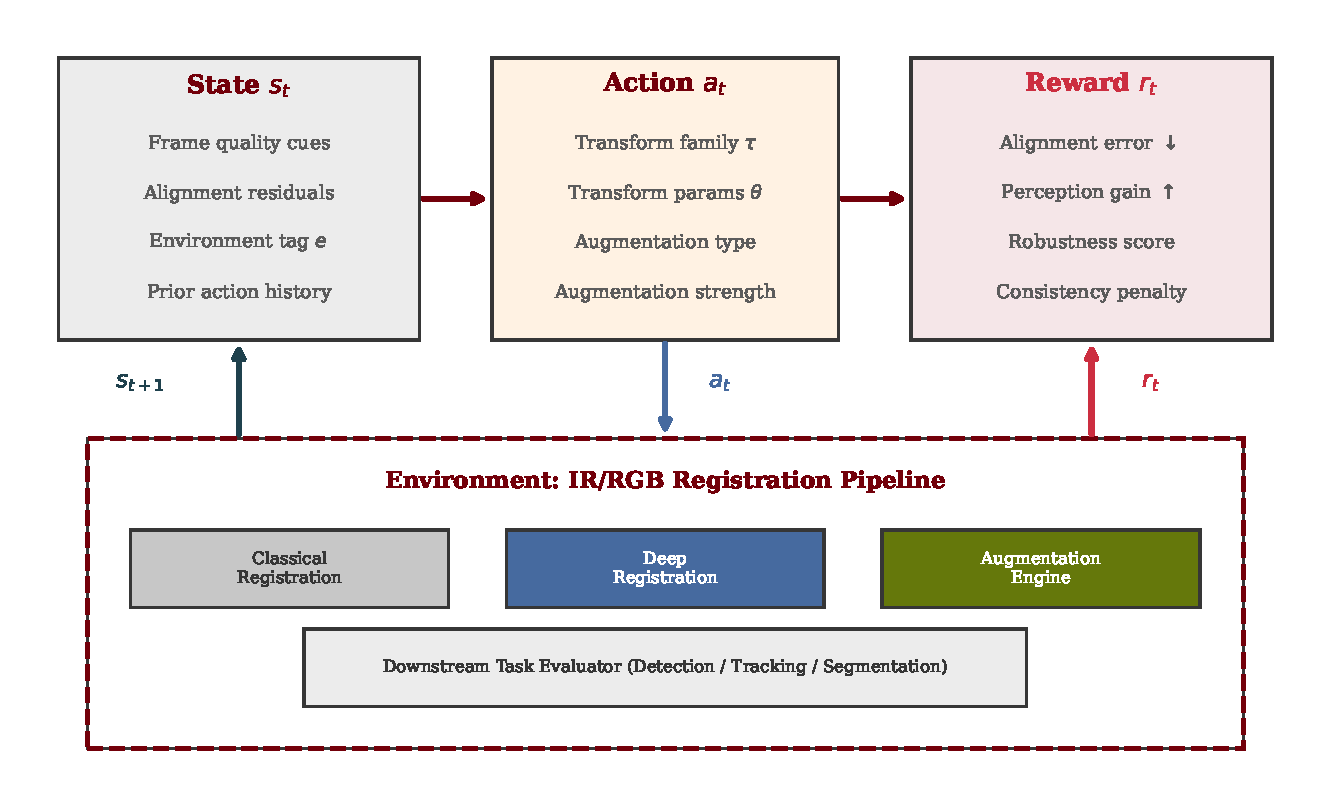
\includegraphics[width=0.95\textwidth]{figures/fig2_rl_loop.pdf}
    \caption{MDP formulation detail. The state $s_t$ encodes frame quality cues, alignment residuals, environment tag, and prior action history. The action $a_t$ specifies both a registration transform (family and parameters) and an augmentation recipe (type and strength). The reward $r_t$ combines alignment error reduction, downstream perception gain, and a consistency penalty.}
    \label{fig:mdp}
\end{figure}

\textbf{State space.} The state $s_t = (q_t, \rho_t, e, h_{t-1})$ consists of four components. Frame quality cues $q_t \in \mathbb{R}^d$ are extracted from both IR and RGB frames using a lightweight feature network, encoding sharpness, contrast, noise level, and cross-modal similarity. Alignment residual proxies $\rho_t \in \mathbb{R}^m$ measure the current registration quality through mutual information estimates and feature correspondence statistics. The environment tag $e \in \{\text{lake}, \text{river}, \text{coast}\}$ is a one-hot encoded domain indicator. The action history $h_{t-1}$ encodes the previous action to enable temporal coherence.

\textbf{Action space.} The action $a_t = (\tau, \theta_\tau, \alpha, \sigma_\alpha)$ is a hybrid discrete-continuous vector. The registration transform family $\tau \in \{\text{rigid}, \text{affine}, \text{projective}, \text{deformable}\}$ is a discrete choice (see Figure~\ref{fig:transforms} for a visual comparison). The transform parameters $\theta_\tau \in \mathbb{R}^{k_\tau}$ are continuous values whose dimensionality depends on the chosen family. The augmentation type $\alpha$ selects from the policy search space (Figure~\ref{fig:augspace}), and the augmentation strength $\sigma_\alpha \in [0, 1]$ controls the magnitude.

\begin{figure}[H]
    \centering
    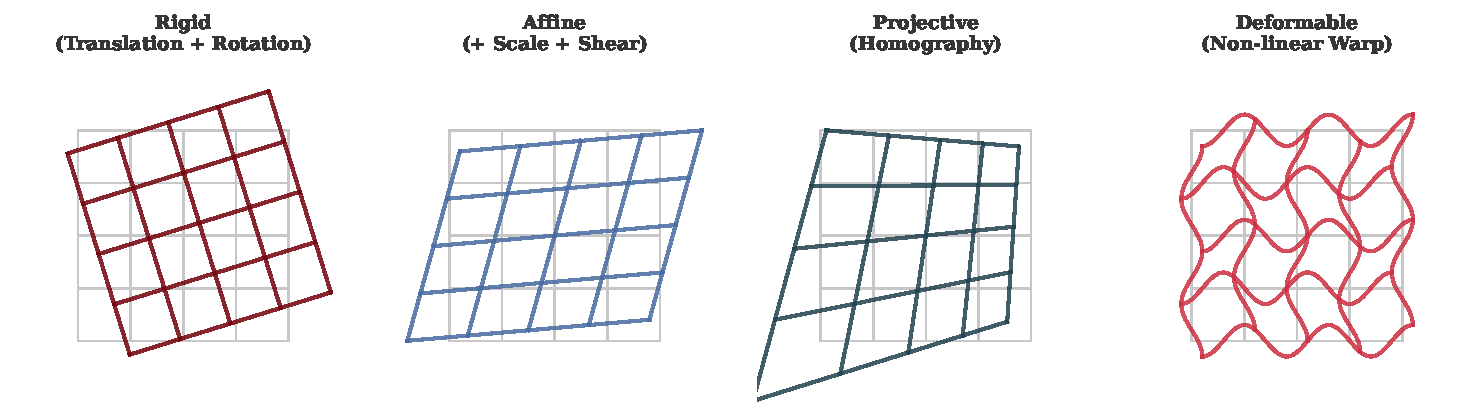
\includegraphics[width=\textwidth]{figures/fig3_transforms.pdf}
    \caption{Registration transform families comprising the discrete component of the action space. From left to right: rigid (translation and rotation, 3 DOF), affine (adds scale and shear, 6 DOF), projective (homography, 8 DOF), and deformable (non-linear warp, dense field). The RL agent selects the family and parameters jointly, adapting complexity to scene requirements.}
    \label{fig:transforms}
\end{figure}

\begin{figure}[H]
    \centering
    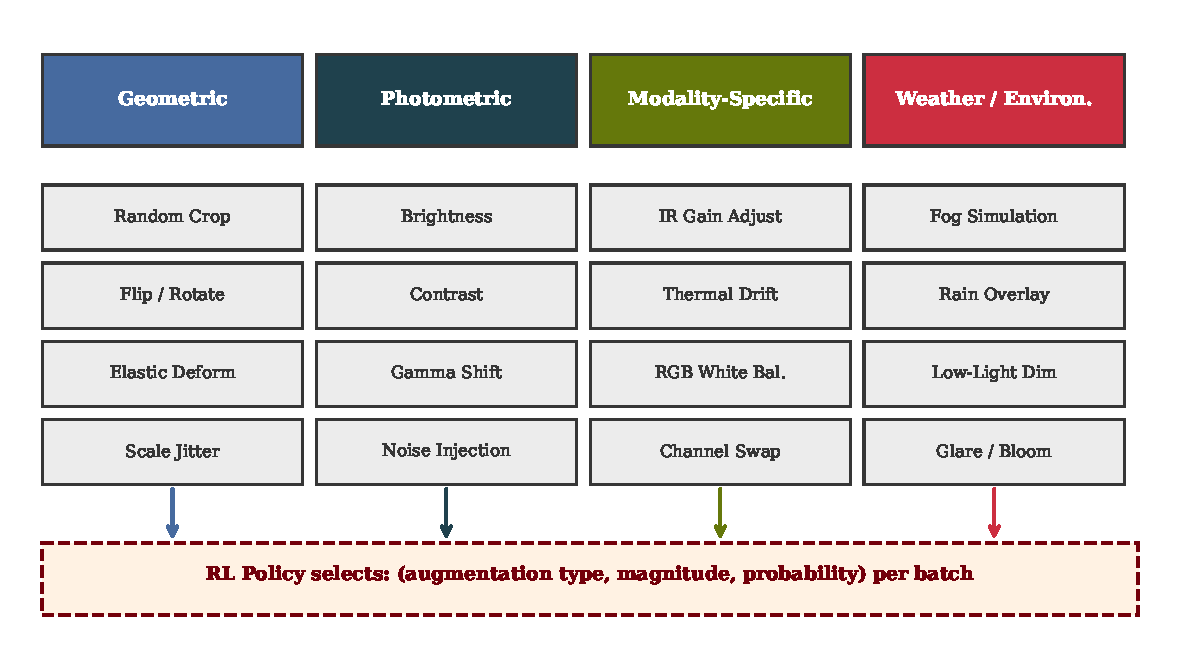
\includegraphics[width=\textwidth]{figures/fig4_augmentation_space.pdf}
    \caption{Augmentation policy search space organized by category. The RL agent selects augmentation type, magnitude, and application probability per training batch. Modality-specific and weather augmentations are unique to our multimodal setting and are not present in standard AutoAugment-style search spaces.}
    \label{fig:augspace}
\end{figure}

\textbf{Reward function.} The reward $r_t$ is a weighted combination of three terms.
\begin{align}
    r_t = \underbrace{w_1 \cdot \Delta F_t}_{\text{perception gain}} - \underbrace{w_2 \cdot \epsilon_t}_{\text{alignment error}} - \underbrace{w_3 \cdot \mathcal{C}_t}_{\text{consistency penalty}}
    \label{eq:reward}
\end{align}
The perception gain $\Delta F_t = F_t - F_{t-1}$ measures improvement in downstream task score (F1 or mAP). The alignment error $\epsilon_t$ penalizes poor registration quality measured by reprojection error on automatically detected correspondences. The consistency penalty $\mathcal{C}_t$ discourages rapid action oscillation by penalizing large changes from $a_{t-1}$ to $a_t$, promoting temporal stability in the selected pipeline configuration.

\subsection{RL Algorithm}

We adopt Soft Actor-Critic (SAC) \citep{Haarnoja2018SAC} as our primary RL algorithm. SAC is well-suited to this problem for three reasons. First, its off-policy nature with experience replay provides sample efficiency, which is critical because each environment step requires running the full registration-train-evaluate loop. Second, the maximum entropy objective $J(\pi) = \mathbb{E}_{s_t}\left[\mathbb{E}_{a_t \sim \pi}\left[\alpha \log \pi(a_t|s_t) - Q(s_t, a_t)\right]\right]$ naturally encourages exploration of diverse registration and augmentation configurations during early training. Third, SAC handles continuous action spaces natively through its stochastic policy. Figure~\ref{fig:sac} illustrates the SAC architecture adapted to our problem.

\begin{figure}[H]
    \centering
    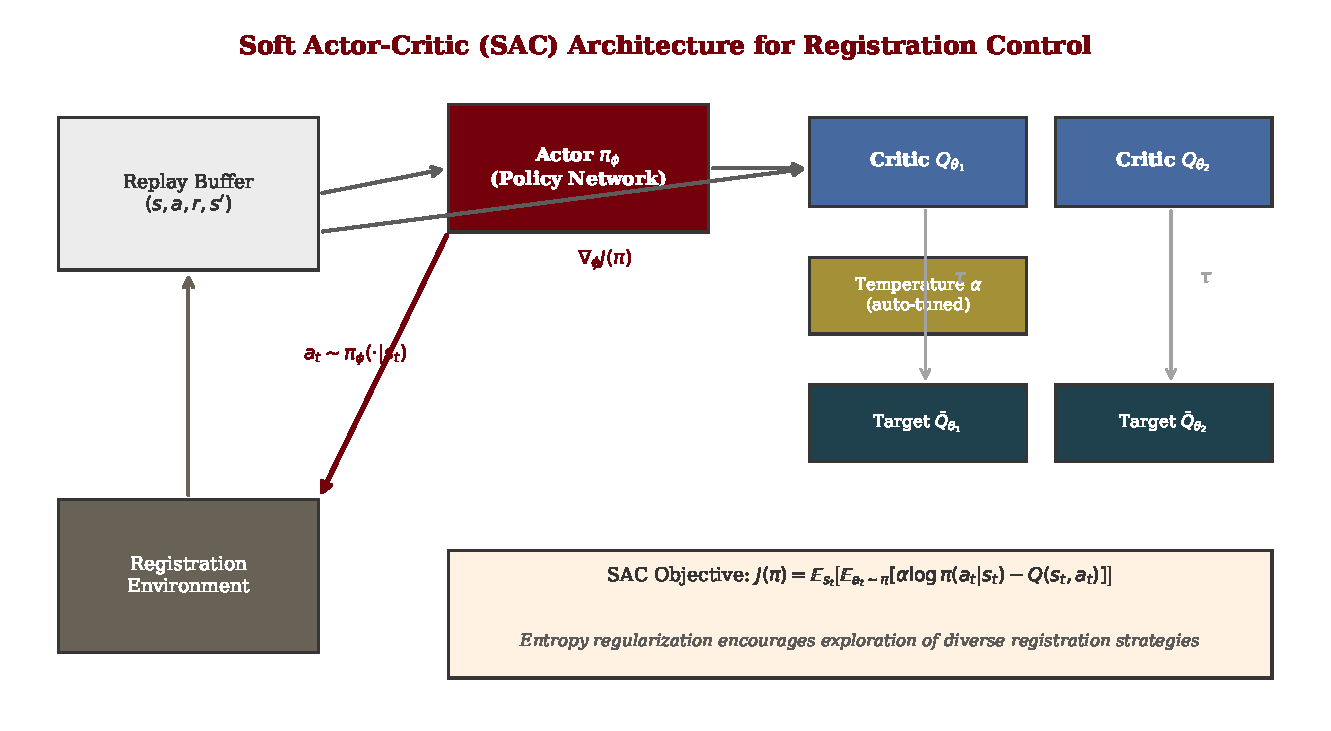
\includegraphics[width=\textwidth]{figures/fig8_sac_architecture.pdf}
    \caption{SAC architecture for registration control. The actor network $\pi_\phi$ maps states to registration and augmentation actions. Twin critics $Q_{\theta_1}, Q_{\theta_2}$ with target networks provide stable value estimates. The automatically tuned temperature $\alpha$ balances exploitation of known good configurations with exploration of novel strategies. Transitions are stored in a replay buffer for off-policy learning.}
    \label{fig:sac}
\end{figure}

For the hybrid discrete-continuous action space, we adopt a factored policy architecture. The discrete transform family selection uses a categorical distribution head, while the continuous parameters use a squashed Gaussian. Both heads share a common feature backbone. We maintain TD3 \citep{Fujimoto2018TD3} as a secondary algorithm for ablation comparison, and PPO \citep{Schulman2017PPO} as an on-policy baseline.

\subsection{Novelty Extensions}

Our approach extends prior work in three key directions.

\textbf{Weather and lighting robustness.} Unlike fixed registration pipelines, our RL policy observes frame quality cues that encode weather-dependent degradation patterns. The agent learns to switch to more robust transform families (e.g., from feature-based affine to dense deformable) under fog or rain, and to apply compensating augmentations (thermal drift simulation, low-light dimming) during training to improve downstream robustness. This is motivated by the observation in Figure~\ref{fig:weather} that modality-specific degradation patterns are highly condition-dependent.

\textbf{Multi-sensor scheduling.} We extend the action space to include a sensor weighting parameter $\omega \in [0, 1]$ that controls the relative contribution of IR versus RGB features in the downstream task. Under clear conditions, RGB may dominate; under night or fog, the agent can shift weight toward IR. This adaptive sensor scheduling is learned end-to-end alongside registration and augmentation.

\textbf{Domain transfer across water bodies.} By conditioning the policy on the environment tag $e$, the agent learns domain-specific registration and augmentation strategies. We evaluate zero-shot transfer by training on two water-body types and testing on the held-out third, measuring whether the environment conditioning enables generalization to unseen domains. Figure~\ref{fig:domain} illustrates this cross-domain evaluation design.

\begin{figure}[H]
    \centering
    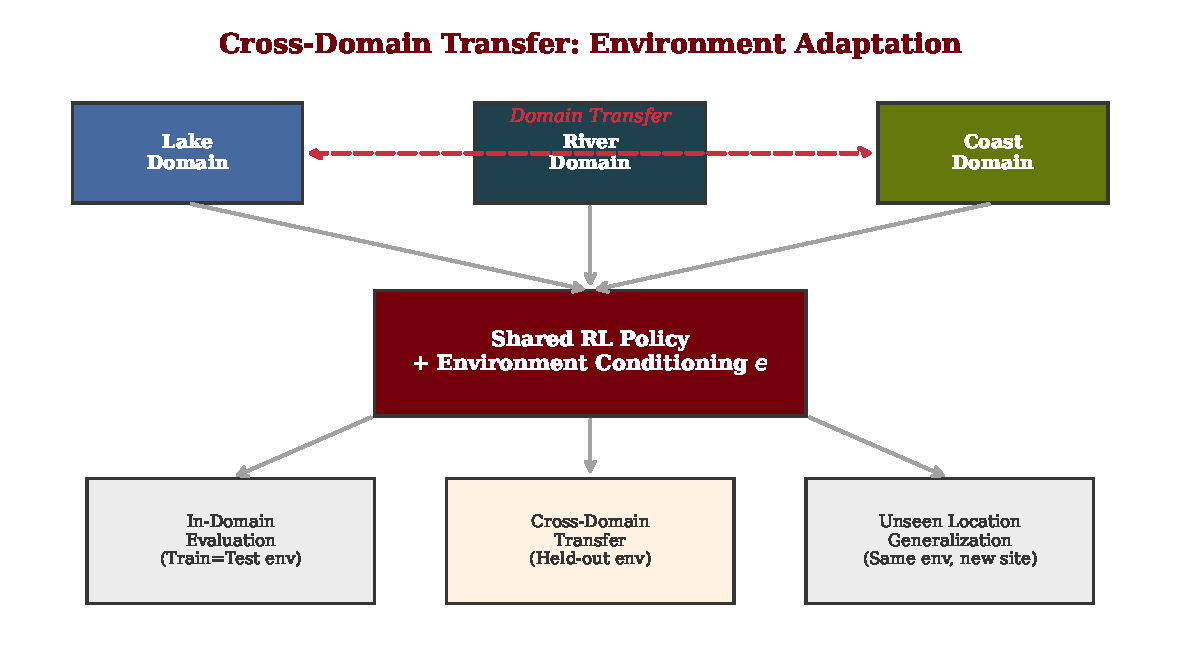
\includegraphics[width=0.9\textwidth]{figures/fig5_domain_transfer.pdf}
    \caption{Cross-domain transfer evaluation design. The shared RL policy is conditioned on environment type $e$ and evaluated in three scenarios: in-domain (train and test on same water body), cross-domain (held-out environment type), and unseen-location (same environment type, new geographic site).}
    \label{fig:domain}
\end{figure}

% ============================================================
% EVALUATION
% ============================================================
\section{Evaluation}

\subsection{Datasets and Splits}

We evaluate on IR/RGB data collected across lake, river, and coastal environments. Data is split by geographic location within each domain to prevent spatial leakage, with 70\%/15\%/15\% train/validation/test partitions. We additionally evaluate on the LasHeR benchmark \citep{Li2022RGBTTracking}, a large-scale RGB-T tracking dataset with diverse scenes, and the RGBT234 benchmark \citep{Li2023IRRegistration} to assess generalization beyond our collected data.

\subsection{Baselines}

We compare against five baselines spanning classical, learned, and RL-free adaptive methods. Table~\ref{tab:baselines} summarizes the comparison.

\begin{table}[H]
    \centering
    \caption{Baseline comparison. Our approach is the only method that jointly optimizes registration transform selection, augmentation policy, and sensor weighting through closed-loop RL.}
    \label{tab:baselines}
    \begin{tabular}{@{}lcccc@{}}
        \toprule
        \textbf{Method} & \textbf{Adaptive Reg.} & \textbf{Adaptive Aug.} & \textbf{Domain Cond.} & \textbf{RL-Based} \\
        \midrule
        Classical Registration & No & No & No & No \\
        Supervised Deep Registration & No & No & No & No \\
        AutoAugment (Non-RL proxy) & No & Yes & No & Yes \\
        Domain-Adversarial Training & No & No & Yes & No \\
        RandAugment & No & Partial & No & No \\
        \textbf{RL Policy (Ours)} & \textbf{Yes} & \textbf{Yes} & \textbf{Yes} & \textbf{Yes} \\
        \bottomrule
    \end{tabular}
\end{table}

\subsection{Metrics}

We report five complementary metrics. \textbf{Alignment error} (mean reprojection error in pixels) measures registration quality. \textbf{Downstream F1 score} and \textbf{mAP} measure perception task performance on the registered and augmented data. \textbf{Robustness score} is the ratio of worst-case to best-case F1 across weather conditions, capturing consistency. \textbf{Cross-domain gap} is the absolute F1 difference between in-domain and cross-domain evaluation, measuring transfer quality.

\subsection{Evaluation Scenarios and Ablations}

We evaluate under four test scenarios of increasing difficulty. \textit{In-domain transfer} trains and tests within the same water-body type. \textit{Cross-domain transfer} trains on two environment types and tests on the held-out third. \textit{Unseen-location robustness} tests on new geographic sites within a known environment type. \textit{Adverse-condition stress testing} evaluates under degraded weather (fog, rain, night). Figure~\ref{fig:expected} shows projected performance trends based on prior work in the constituent subproblems.

\begin{figure}[H]
    \centering
    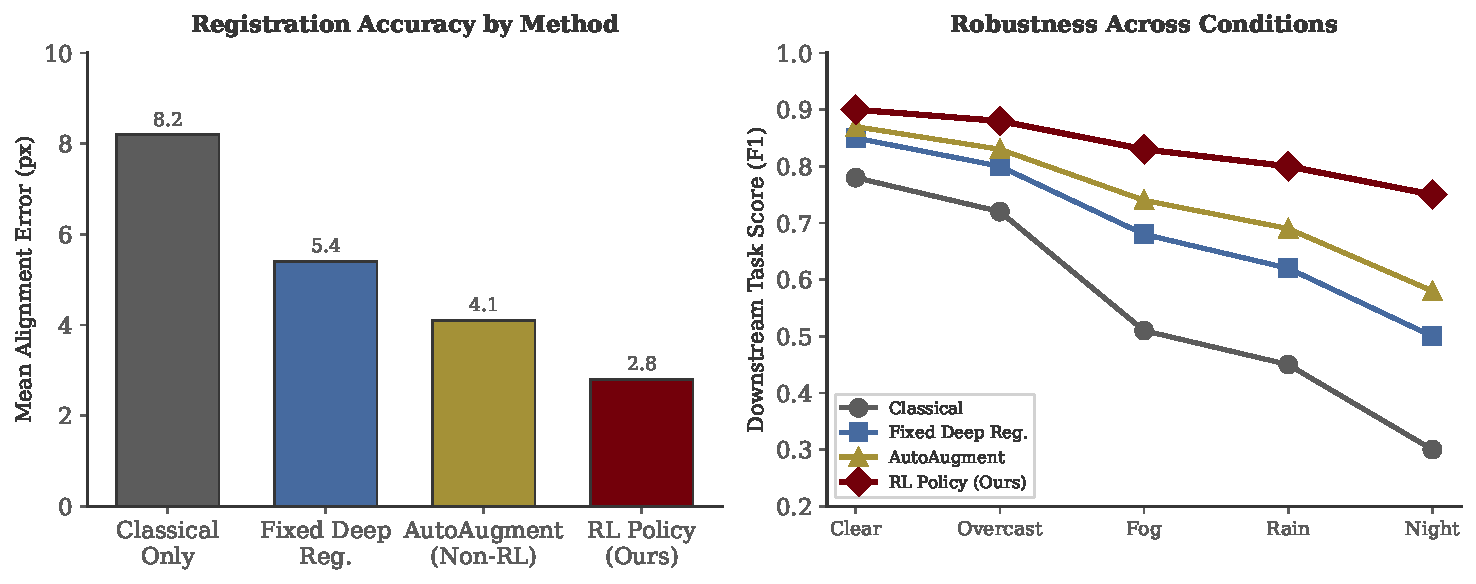
\includegraphics[width=\textwidth]{figures/fig6_expected_results.pdf}
    \caption{Projected performance based on trends in prior work. Left: alignment error by method, showing expected improvement from classical through RL-optimized registration. Right: downstream F1 score across weather conditions, illustrating the robustness advantage of adaptive RL-based selection over fixed pipelines. Values are estimates based on related work baselines.}
    \label{fig:expected}
\end{figure}

We additionally conduct three ablation studies. First, we remove the RL loop entirely (fixed registration and augmentation) to measure the contribution of adaptive selection. Second, we remove environment conditioning to isolate the benefit of domain-specific policy heads. Third, we compare SAC against TD3 and PPO to evaluate algorithm sensitivity.

% ============================================================
% CONCLUSION
% ============================================================
\section{Conclusion}

We propose a reinforcement learning framework that jointly optimizes IR/RGB image registration and data augmentation for downstream multimodal perception. By formulating the problem as an MDP where a SAC-trained policy selects registration transforms, augmentation recipes, and sensor weighting conditioned on frame quality, alignment residuals, and environment type, our approach replaces rigid hand-designed pipelines with a closed-loop adaptive system. The evaluation plan spans in-domain, cross-domain, unseen-location, and adverse-condition scenarios, compared against classical registration, supervised deep registration, AutoAugment, domain-adversarial training, and RandAugment baselines across alignment error, downstream F1/mAP, robustness score, and cross-domain gap metrics. Three novelty extensions---weather-adaptive registration, learned sensor scheduling, and domain-conditioned transfer---push beyond existing work in both RL for registration and RL for augmentation. The framework leverages existing IR/RGB datasets and runs on available compute (2 servers with 4$\times$ RTX 6000 Ada each), making it feasible within a single semester.

% ============================================================
% REFERENCES
% ============================================================
\bibliography{references}
\nocite{*}

\end{document}
